% 2006 天津文科 Q19，源：固定 PDF 第 1 页（印刷页 338）。
% 节点：A,B,C,D 为矩形 ABCD 的角点，O 为对角线交点；E,F 为等边三角形 CDE
% 的第三顶点与棱端点。识别的实线：BC, CD, DE, EF, FB, EC, FC。
% 识别的虚线：AB, AD, AF, FO, EO, FD。题干说 O 是矩形 ABCD 对角线交点，
% 但源图未画 AC/BD 对角线，故未补画；O 是 FO 与 EO 两条虚线的端点。
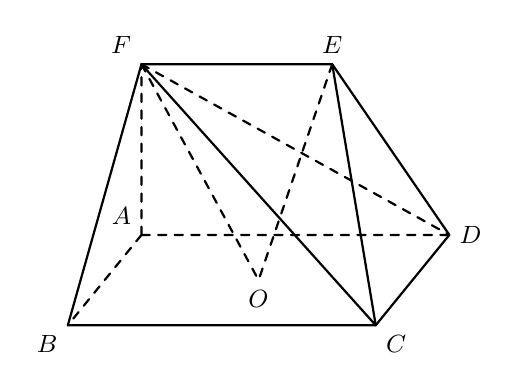
\begin{tikzpicture}[x=0.85cm,y=0.85cm,line cap=round,line join=round,line width=0.8pt,font=\small]
  \coordinate (A) at (1.1,1.35);
  \coordinate (B) at (0,0);
  \coordinate (C) at (4.6,0);
  \coordinate (D) at (5.7,1.35);
  \coordinate (O) at (2.85,0.675);
  \coordinate (F) at (1.1,3.9);
  \coordinate (E) at (3.95,3.9);
  % 隐藏棱与辅助虚线
  \draw[dashed] (A)--(B) (A)--(D) (A)--(F);
  \draw[dashed] (F)--(O) (E)--(O) (F)--(D);
  % 可见棱及内部实线
  \draw (B)--(C)--(D)--(E)--(F)--(B);
  \draw (E)--(C) (F)--(C);
  \node[above left] at (A) {$A$};
  \node[below left] at (B) {$B$};
  \node[below right] at (C) {$C$};
  \node[right] at (D) {$D$};
  \node[above] at (E) {$E$};
  \node[above left] at (F) {$F$};
  \node[below] at (O) {$O$};
\end{tikzpicture}
